% rapport.tex
% Template LaTeX pour un rapport scientifique (conservation du hérisson)
% Compile: pdflatex rapport.tex -> biber rapport -> pdflatex rapport.tex (ou use latexmk -pdf)

\documentclass[a4paper,11pt]{article}
\usepackage[T1]{fontenc}
\usepackage[utf8]{inputenc}
\usepackage[french]{babel}
\usepackage{microtype}
\usepackage{geometry}
\geometry{left=25mm,right=25mm,top=25mm,bottom=25mm}
\usepackage{graphicx}
\usepackage{caption}
\usepackage{subcaption}
\usepackage{booktabs}
\usepackage{csquotes}
\usepackage[style=apa,backend=biber,sorting=nyt]{biblatex}
\DeclareLanguageMapping{french}{french-apa}
\addbibresource{refs.bib}
\addbibresource{sources_web.bib}
\usepackage{hyperref}
\hypersetup{colorlinks=true,linkcolor=blue,citecolor=blue,urlcolor=blue}
\usepackage{siunitx} % unités
\usepackage{float}
\usepackage{enumitem}
\usepackage{etoolbox}
\usepackage{lineno}
\usepackage{setspace}
%\onehalfspacing
\doublespacing
\lefthyphenmin=3
\righthyphenmin=3
\setlength{\parindent}{0pt}
\setlength{\parskip}{0.5\baselineskip plus 0.1\baselineskip minus 0.1\baselineskip}
\pretocmd{\section}{\clearpage}{}{}


% -------------------------------------------------------------------

% Informations du document
\title{Conservation du hérisson : rapport scientifique}
\author{Prénom NOM \\ ULB - Bachelier en Bioingénieur}
\date{\today}

\begin{document}
\pagenumbering{roman}
\maketitle

\section*{Licence}

Ce document est mis à disposition sous licence Creative Commons Attribution 4.0 International (CC BY 4.0).

© 2026 LES6PICS

\tableofcontents
\newpage

\linenumbers

\section{Introduction}
\pagenumbering{arabic}
Les enjeux liés à la biodiversité occupent aujourd’hui une place croissante dans le débat public. Cette mobilisation n’est toutefois pas récente : dès le début des années 1990, la communauté internationale s’est engagée dans la protection du vivant, notamment avec l’adoption de la Convention des Nations Unies sur la diversité biologique (Secretariat of the Convention on Biological Diversity, 2025).

Malgré ces engagements, l’érosion de la biodiversité se poursuit. Selon l’édition 2025 de la Liste rouge de l’IUCN (Union internationale pour la conservation de la nature), plus de 48 600 espèces sur les 172 620 évaluées, soit 28\%, sont actuellement menacées d’extinction (The IUCN Red List of Threatened Species, 2025).

Dans l’imaginaire collectif européen, cette crise est souvent associée à la disparition de grands mammifères exotiques, tels que les tigres, les lions ou les rhinocéros. Pourtant, elle touche aussi des espèces beaucoup plus proches de notre quotidien.

En Europe, au moins 1 677 espèces, soit 11\% des espèces évaluées par l’IUCN, sont menacées d’extinction (The IUCN Red List of Threatened Species, 2025).

Notre projet s’est intéressé au hérisson européen (Erinaceus europaeus), une espèce largement appréciée du public mais encore insuffisamment étudiée et documentée, notamment en ce qui concerne l’état de sa population. E. europaeus est un petit mammifère nocturne insectivore de la famille des érinacéidés (Erinaceidae). Reconnaissable à ses piquants, le hérisson est reconnu pour son rôle d’espèce parapluie, c’est-à-dire que sa protection permet de maintenir de nombreuses autres espèces animales (amphibiens, insectes, petits mammifères) ainsi que la flore, qui partagent le même habitat (Roberge et al., 2004). En plus de ce rôle, il contribue à la régulation des invertébrés et à l’équilibre de son écosystème.

Le hérisson voit sa population reculer dans plusieurs régions du continent européen (Gazzard et al., 2025). Les causes sont multiples. Parmi celles-ci, on peut citer: fragmentation croissante des habitats, urbanisation, intensification agricole, usage massif de pesticides ou encore mortalité routière (figure 1). Ces pressions cumulées fragilisent davantage cette espèce caractérisée par une hibernation sensible aux perturbations, la saisonnalité de sa reproduction, une faible capacité de dispersion, ainsi qu’une sensibilité accrue face à certaines maladies. Autant de traits qui limitent sa résilience face aux changements environnementaux. Cette situation a récemment conduit l’IUCN (The IUCN Red List of Threatened Species, 2025) à revoir le classement du hérisson européen, qui passe de la catégorie \enquote{préoccupation mineure} à la catégorie des espèces \enquote{quasi menacées}, reflétant une inquiétude croissante quant à son avenir à l’échelle continentale (The IUCN Red List of Threatened Species, 2012).

Dans le cadre de notre projet, nous nous sommes intéressés à la situation en Belgique. Alors que la Flandre dispose déjà d’un certain volume de données, la Wallonie reste marquée par un manque d’informations structurées, qui complique fortement l’évaluation de l’état réel des populations (figure 2). Ce déficit constitue un frein majeur à l’élaboration de stratégies de conservation cohérentes et adaptées.

Pour répondre à cette question, nous avons passé en revue les données disponibles en Flandre, au Luxembourg, dans certaines régions de France ainsi qu’en Wallonie. Nous avons également étudié les méthodes de recensement mises en œuvre par les différents acteurs et analysé les outils mobilisés à cette fin. L’objectif était d’identifier les dispositifs les plus efficaces et d’évaluer dans quelle mesure ils pourraient être adaptés au contexte wallon. Parallèlement, nous avons rassemblé des informations sur la biologie générale du hérisson, jugées indispensables pour mieux comprendre l’espèce et orienter sa protection.

Nous avons ensuite examiné les causes du déclin, ses conséquences environnementales et socio-économiques, ainsi que les solutions envisageables pour y répondre. L’ensemble de ce travail repose principalement sur des articles scientifiques, des sites naturalistes et des rapports institutionnels, complétés par l’exploration de plateformes de recensement déjà existantes.

Cette démarche nous a conduits à proposer un dispositif de collecte d’observations géoréférencées destiné à compléter le travail d’inventaire des professionnels. Plus simple d’utilisation que les outils actuels, il vise à élargir la participation citoyenne et, à terme, à soutenir plus efficacement la conservation de l’espèce en Wallonie.

\section{Recherches bibliographiques sur la biologie du hérisson}

Comme indiqué dans l’introduction, nous présentons d’abord les principaux éléments de biologie du hérisson. Cette étape est indispensable pour comprendre en quoi son mode de vie, ses besoins écologiques et son rythme saisonnier influencent sa vulnérabilité face aux pressions actuelles.

\subsection{Espèce parapluie}

Le hérisson est souvent présenté comme une espèce parapluie, c’est-à-dire une espèce dont la protection bénéficie indirectement à de nombreuses autres. Ce statut repose généralement sur plusieurs caractéristiques : un territoire relativement étendu, des exigences écologiques marquées et une sensibilité aux perturbations du milieu (Nature, s. d. ; Espèce PARAPLUIE - Définition et exemples, s. d.). Protéger une telle espèce revient donc à préserver, au moins en partie, les habitats et les ressources dont dépendent d’autres organismes.

Le hérisson partage plusieurs de ces caractéristiques. Son domaine vital peut être relativement large à l’échelle d’un petit mammifère, il dépend d’habitats offrant à la fois nourriture et refuges, et il réagit fortement à la dégradation de son environnement. À cela s’ajoute un autre élément important : le hérisson bénéficie d’une image très positive auprès du grand public, ce qui en fait également une espèce porteuse en matière de sensibilisation. Cette double dimension, écologique et symbolique, renforce l’intérêt de sa conservation.

\subsection{Caractéristiques physiques}
Le hérisson commun ou, de son nom latin, Erinaceus europaeus est un petit mammifère appartenant à la famille des érinacéidés. Il mesure en général entre 22 et 28cm de longueur pour 12 à 15cm de hauteur, son poids oscille de 600 à 1500 grammes en fonction des saisons et des conditions alimentaires (hérisson - Dictionnaire des Sciences Animales, s. d.) (Haigh et al., 2012). Le phénotype de ce petit mammifère est principalement caractérisé par une apparence trapue et des piquants sur la majorité du corps. A l’apex de sa tête, on peut observer un museau pointu et fin aussi appelé rhinophore qui est suivi de petits yeux et d’oreilles courtes et rondes, et qui constituent ensemble la tête du hérisson. S’en suit le tronc du hérisson qui est relativement trapu et qui se termine par une queue qui peut atteindre jusqu’à 6cm (hérisson - Dictionnaire des Sciences Animales, s. d.). Celle-ci est partiellement cachée par les piquants longs et denses qui recouvrent la majorité de son corps. Les piquants sont creux et atteignent environ 2 à 3cm . Ils sont souvent associés à tort à des épines mais sont en fait des poils durs et creux, faits de kératine, ce qui les rend à la fois solides et légers (Études de Li (2022) et Kennedy (2017)). Un hérisson adulte en possède entre 5000 et 6000 qui sont renouvelés tous les 18 mois. Les piquants sont bicolores, clairs à leur base et leur extrémité et plus foncés en leur milieu, ce qui rend la silhouette du hérisson moins structurée. Ils ont un rôle protecteur majeur contre les prédateurs mais ne constitue pas un atout contre les pressions émergentes que nous allons détailler plus tard. Le hérisson est un quadripède, ces 4 pattes sont fines et courtes et chacune munies de griffes. Les pattes avant sont légèrement plus courtes que les pattes arrière et sont adaptées à la recherche de ses proies dans le sol. 

\subsection{Mode de vie et comportement}
Cette espèce présente une activité nocturne, c’est-à-dire qu’ils sont majoritairement actifs la nuit. Cette caractéristique leur permet d’éviter les prédateurs aériens diurnes. En journée, ils se réfugient sous de la végétation, dans des crevasses ou parfois dans des terriers (Hedgehog | Small Mammal, Nocturnal Habits \& Spines | Britannica, 2026). Aussi, les hérissons sont solitaires, les interactions interspécifiques sont donc rares, excepté pendant la saison de reproduction.

\subsection{Alimentation}
De plus, ces petits mammifères sont opportunistes, ils se nourrissent dès que des ressources sont disponibles dans leur environnement (Nesting Behaviour and Seasonal Body Mass Changes in a Rural Irish Population of the Western Hedgehog (Erinaceus Europaeus), s. d.). Cependant, on observe chez le hérisson une tendance marquée pour le régime insectivore. Leur régime alimentaire est dès lors constitué d’une gamme très variée d’insectes. On y retrouve par exemple des scarabées, des arthropodes, des coléoptères ou des perces oreilles. Aussi, le hérisson se nourrit d’invertébrés comme des vers de terres, des millepattes ou bien encore des limaces. En plus de ces derniers, on retrouve parfois des proies vertébrées comme des oisillons (ou encore des œufs), des petits reptiles, des fruits ou des champignons (O¨ zen, 2006), bien que ces derniers restent des apports nutritifs secondaires et rares pour le hérisson (Yalden, 1976.). Comme énoncé précédemment, le hérisson est opportuniste, la disponibilité des ressources variant avec les saisons, le poids des hérissons suit la même tendance, avec un poids plus élevé à la fin de la saison chaude pratique car les hérissons doivent accumuler des graisses pour pouvoir tamponner leur perte de poids dû à l’hibernation en hiver (Haigh et al., 2012).

\subsection{Habitat}
Le hérisson affectionne particulièrement les lisières boisées, les haies, les jardins et les zones herbacées. La distribution spatiale de l’espèce est directement liée à l’abondance des ressources alimentaires offertes par son environnement. Les haies sont le milieu favori des hérissons. En plus de leur offrir un endroit riche en ressources, les haies leur offrent une protection naturelle et efficace contre les prédateurs aériens (Haigh et al., 2012). Or, avec l’intensification de l’agriculture, les paysages agricoles changent et les espaces autrefois réservoirs à biodiversité grâce aux haies laissent place à des paysages de plus en plus homogène qui limitent notamment la survie des hérissons. 

\subsection{Comportement de chasse}
La chasse se fait par la technique du foraging qui est d’ailleurs considérée comme la méthode la plus chronophage pour les animaux nocturnes (Haigh et al., 2012). Celle-ci consiste en la recherche nocturne de proie dans le sol ou sous la végétation à l’aide de l’odorat. Elle est rendue possible car ce sens est particulièrement développé chez le hérisson (Adrian, 1942). En effet, le rhinophore, joue un rôle sensoriel essentiel : il lui permet de détecter les odeurs et les vibrations du sol pour repérer ses proies. La morphologie des pattes du hérisson et celle de ses griffes sont adaptées à la fouille dans le sol et sont donc un avantage pour la chasse.

\subsection{Stratégie de survie (vide)}

\subsection{Prédateurs}
Ses prédateurs naturels sont les blaireaux, les renards ou encore certains rapaces (Doncaster, 1993). La nocturnité des hérissons leur permet d’éviter les prédateurs aériens. Lorsqu'ils se sentent menacés, les hérissons se roulent en boule, ce qui protège leurs parties vulnérables grâce à leurs piquants. Ce comportement est leur mécanisme de défense principal auquel ils peuvent ajouter la production d’un bruit strident pour repousser les prédateurs. 

\subsection{Maladies et parasites (vide)}

\subsection{Mortalité}
Aujourd’hui, en plus de la prédation naturelle, de nouveaux dangers sont apparus pour cette espèce. On peut notamment citer les collisions routières, les tondeuses ou encore les produits phytosanitaires desquels les piquants du hérisson ne peuvent pas les protéger. Une autre cause de mortalité chez cette espèce est leur vulnérabilité face à diverses maladies, liées à des parasites externes (tiques, puces) ou internes (nématodes, coccidies), ainsi qu’à des virus comme le Capillaria (Rautio et al., 2016). La fraction de hérissons atteints de maladie croit avec la concentration d’individus et la proximité de l’homme qui favorisent la propagation de ces pathologies.

Les hérissons sont des mammifères avec une longévité pouvant atteindre les 10 ans lorsque les conditions sont optimales et que les facteurs externes (manque de nourriture, prédation, maladies) sont éloignés. En réalité, la longévité de ce petit mammifère dépasse rarement deux ans dans la nature. En effet, la première hibernation fait souvent des ravages chez les jeunes hérissons, si bien qu'environ 50\% n’atteignent pas la 2e année. Rares sont les hérissons atteignant les 5 ans à l’état sauvage. Ce haut taux de mortalité peut être lié au manque de nourriture, aux maladies ou encore à la prédation naturelle et tend à croître avec l’intensification des pressions émergentes.

\subsection{Reproduction}
La période de reproduction des hérissons s’étend généralement d’avril à septembre, mais peut dépasser ces dates et commencer dès la fin de l’hibernation quand les conditions climatiques s’y prêtent. Les mâles en quête de partenaire, peuvent parcourir de longues distances pour trouver une femelle, qu’ils séduisent pour se reproduire. Une fois l’accouplement terminé, les mâles repartent à la recherche d’une nouvelle femelle tandis que la femelle gestante s’active pour préparer l’arrivée de ses hérisonnets environ 35 jours plus tard. Les portées sont d’environ 5 petits, qui naissent aveugles et sourds. La vue et l’odorat ne se développent que quelques jours après. 

\subsection{Hibernation}
L’hibernation commence généralement dès la fin de septembre, au début de l’hiver et se termine à la fin mars. Les ressources en nourriture diminuent, les températures chutent et les jours se rallongent ce qui poussent le hérisson à commencer son hibernation. Pour cela, le hérisson se prépare un abri pour passer cette période. Pendant l’hibernation, toutes les constantes vitales (température, respiration, rythme cardiaque) du hérisson baissent lui permettant de consommer le moins d’énergie possible et donc de perdre le moins de poids possible. Malgré cela, le quadripède perd en moyenne 20 à 40\% de son poids corporel initial. (est ce qu’il faut parler du fait que les males hibernent plus tôt que les femelles ? Est-ce qu’on parle aussi des interruptions pendant l’hibernation ? => est ce que ça explique une partie des morts sur route en hiver ?) 

\section{Causes et conséquences du déclin du hérisson}

\subsection{Fragmentation des habitats}

Les hérissons, notamment le hérisson européen (Erinaceus europaeus), sont fortement impactés par la fragmentation des habitats et l’urbanisation, qui modifient leurs déplacements, leurs ressources et leurs sites de nidification. Dans les paysages morcelés, ils tendent à parcourir de plus grandes distances et à se déplacer plus rapidement pour accéder à la nourriture, aux abris et aux partenaires, ce qui illustre une certaine plasticité comportementale face à la dégradation de l’habitat (Berger et al., 2020).

\subsection{Urbanisation et exil vers les villes}

On observe aujourd’hui un déplacement progressif des hérissons des milieux ruraux vers les zones urbaines et périurbaines, où ils trouvent encore de la nourriture, des abris et des jardins relativement favorables. Ce \enquote{refuge urbain} reste toutefois ambivalent : il résulte de la dégradation de leurs habitats traditionnels (intensification agricole, pesticides, disparition des haies) et s’accompagne de nouveaux risques en ville (trafic routier, clôtures, dérangements), ce qui justifie de mettre en avant, dans un rapport de conservation, la nécessité de préserver et connecter les jardins, parcs et espaces verts comme zones clés pour la survie des hérissons. En zones périurbaines, ils utilisent préférentiellement les espaces verts connectés (haies, jardins, boisements) et évitent les zones à forte présence humaine ou à forte circulation, soulignant l’importance de la connectivité écologique (Sánchez et al., 2023).

\subsection{Réchauffement climatique}

Le réchauffement climatique et l’urbanisation influencent également l’hibernation. Chez les hérissons vivant en climat tempéré, la période d’hibernation présente une grande variabilité individuelle, tant pour le début que pour la fin, ce qui suggère une capacité d’ajustement aux années plus douces ou plus irrégulières (Journal of Thermal Biology, 2025). La présence de nourriture artificielle en milieu urbain peut cependant perturber ces rythmes, en maintenant certains individus actifs plus longtemps en hiver et en modifiant leur physiologie saisonnière (Gazzard \& Baker, 2020). Par ailleurs, l’utilisation de structures et de matériaux urbains pour la construction des nids illustre une adaptation aux environnements anthropisés, mais les effets à long terme sur la survie hivernale restent encore mal connus.

\subsection{Hibernation sensible}

L’hibernation commence généralement à l’automne, lorsque les températures baissent et que les jours raccourcissent, et se prolonge jusqu’au printemps. Elle se caractérise par des cycles de torpeur et de réveil, dont la durée et la fréquence varient selon les individus, ce qui pourrait constituer une réponse à des hivers de plus en plus imprévisibles (Journal of Thermal Biology, 2025). Ce repos hivernal est étroitement intégré au cycle de vie : sa durée et son calendrier conditionnent l’état corporel à la sortie d’hibernation et donc la capacité à se reproduire.

\subsection{Saisonnalité de la reproduction}

La reproduction est saisonnière, avec un début généralement situé après la fin de l’hibernation. Les femelles sont fécondées au printemps et les naissances se concentrent vers la fin du printemps et le début de l’été, période qui coïncide avec une forte disponibilité en proies (Natural History Museum, s.d.)(Animal Diversity Web, s.d.). La photopériode constitue un signal environnemental majeur pour synchroniser ces cycles : elle influence la sécrétion d’hormones impliquées dans l’activation du système reproducteur, notamment chez le mâle (Saboureau et al., 1993). Chez les femelles, la thermorégulation durant la saison de reproduction reflète un coût énergétique élevé lié à la gestation et à l’élevage des jeunes (Kowalski \& Rzasa, 1988).

De manière générale, le cycle de vie des hérissons repose sur une alternance entre une phase d’activité (alimentation, reproduction, dispersion) et une phase d’hibernation, toutes deux fortement dépendantes de la qualité et de la connectivité des habitats. La fragmentation, l’urbanisation et le réchauffement climatique perturbent ces rythmes naturels en modifiant les paysages, les ressources disponibles et les signaux saisonniers. Ces perturbations peuvent fragiliser les populations et renforcent l’importance des actions de conservation et de suivi afin d’adapter les mesures de protection.

\subsection{Impacts socio-économiques}

En Belgique, le hérisson d’Europe (Erinaceus europaeus) bénéficie d’une protection stricte tant au niveau fédéral que régional (Wallonie, Flandre et Bruxelles). Toute capture, détention, mise à mort, perturbation intentionnelle ou commerce de l’espèce est strictement interdite, notamment en Région wallonne (Parlement wallon, 2024). Il n’existe aucun marché légal pour les hérissons vivants ni pour leurs produits dérivés, ce qui exclut toute valorisation économique directe. Les coûts liés à sa conservation reposent essentiellement sur les centres de soins et de revalidation, financés par des associations et les pouvoirs publics.

Au-delà de cette protection réglementaire, le hérisson apporte une valeur écologique indirecte significative en tant que prédateur naturel de limaces, escargots et insectes nuisibles. Il constitue ainsi un allié gratuit pour le jardinage biologique et la petite agriculture, contribuant à réduire l’usage de pesticides et d’appâts anti-limaces dans les jardins privés et les zones périurbaines (Bien-être animal Wallonie, s.d.). Bien que ce service écosystémique ne soit pas précisément chiffré, il génère des bénéfices économiques indirects pour les ménages et les exploitations agricoles pratiquant une gestion raisonnée (LRBPO, s.d.-b).

Cependant, l’espèce connaît un déclin préoccupant. Elle est classée comme \enquote{quasi-menacée} sur la Liste rouge de l’UICN depuis octobre 2024 (après avoir été considérée en \enquote{préoccupation mineure}), l’espèce affiche des baisses locales pouvant atteindre 50 \% en Flandre et une tendance générale de 16 à 33 \% sur dix ans en Europe de l’Ouest (UICN, 2024 ; RTBF, 2024a). En trente ans, au moins 40 \% de la population européenne aurait disparu, avec un impact particulièrement marqué en Belgique (RTBF, 2024b). Ce déclin engendre plusieurs coûts socio-économiques. Les collisions routières constituent la première cause de mortalité anthropique, ainsi que la fragmentation des habitats. De plus, l’utilisation de pesticides, le déclin des populations d’insectes, l’urbanisation croissante et l’intensification agricole contribuent à la disparition des haies et du bocage, entraînant des coûts sociétaux liés à la dégradation de la biodiversité, à la santé publique et à la nécessité de mesures compensatoires en agroécologie (LRBPO, 2021.) (LRBPO, s.d.-b). Ces phénomènes font l’objet d’un suivi national depuis 2021 par la Ligue Royale Belge pour la Protection des Oiseaux (LRBPO), qui inclut le marquage et le suivi post-soins des individus afin d’évaluer leur taux de survie (LRBPO, 2021.).

Enfin, le hérisson bénéficie en Belgique d’une forte dimension sociale et culturelle. Symbole très apprécié du public, il jouit d’une sympathie élevée qui favorise une acceptabilité importante des mesures de protection. De nombreux citoyens participent activement à l’étude \enquote{Suivi Hérisson} de la LRBPO via des observations et signalements, aménagent leurs jardins (passages de 13-15 cm sous les clôtures, coins sauvages, bandes herbeuses) et limitent l’usage des robots-tondeuses nocturnes ou des pesticides (LRBPO, s.d.) (Bien-être animal Wallonie, s.d.). Certaines communes, comme Namur, ont adopté des réglementations spécifiques limitant l’utilisation des robots-tondeuses afin de protéger les hérissons actifs la nuit. Cette mobilisation citoyenne, soutenue par les associations, représente un atout majeur : elle implique un coût individuel faible mais une forte implication collective en faveur de la biodiversité urbaine et périurbaine.

En résumé, si le hérisson ne génère aucune économie directe en Belgique, sa conservation présente des bénéfices écologiques indirects non négligeables et s’appuie sur une acceptabilité sociale élevée. Son déclin rapide constitue cependant un coût socio-économique tangible, illustrant la crise de la biodiversité en milieux urbanisés et agricoles, tout en suscitant une réponse citoyenne active via les associations de protection de la nature (UICN, 2024.) (RTBF, 2024a.) (LRBPO, 2021.).

\subsection{Associations et protection du hérisson}

En Belgique, la protection et les soins des hérissons (Erinaceus europaeus) reposent principalement sur un réseau de centres de réhabilitation agréés pour la faune sauvage. Il n'existe pas d'association nationale dédiée exclusivement aux hérissons, mais plutôt des structures régionales qui se spécialisent sur cette espèce ou les accueillent avec d’autres animaux. Ils accueillent souvent des centaines voire des milliers d’hérissons par an au niveau national. Les hérissons sont une espèce protégée, et leur prise en charge doit donc se faire via ces centres reconnus.

\subsubsection{En Wallonie et à Bruxelles (région francophone)}

La Wallonie compte une dizaine de CREAVES (Centres de Revalidation des Espèces Animales Vivant à l’État Sauvage), coordonnés notamment par la Ligue Royale Belge pour la Protection des Oiseaux (LRBPO). Deux centres se distinguent par leur spécialisation exclusive sur les hérissons :

\paragraph{Le Chalet des Hirchons (Quaregnon, près de Mons, province de Hainaut)}

C’est un Centre CREAVES dédié uniquement aux hérissons. Il a accueilli 947 hérissons rien qu'en 2025. Il gère les cas de déshydratation, blessures (tondeuses, routes), jeunes orphelins ou animaux affaiblis avant l'hibernation.

Site : chaletdeshirchons.be

\paragraph{CREAVES \enquote{Les N’hérissons} (Sprimont, province de Liège)}

Également spécialisé sur les hérissons. Il est très réputé en province de Liège pour son expertise sur cette espèce.

D'autres CREAVES accueillent régulièrement un grand nombre de hérissons parmi d'autres espèces sauvages : CREAVES de Namur (devenu un \enquote{hôpital pour la faune sauvage} en 2026, avec zone dédiée aux hérissons); Le Martinet (Theux); ECentre de Soins pour la Faune Sauvage de Bruxelles (Anderlecht, géré par la LRBPO, très actif en région bruxelloise).

La LRBPO joue un rôle clé via son projet \enquote{Suivons nos hérissons} (suivi scientifique par baguage) et sa liste actualisée des centres : protectiondesoiseaux.be/les-centres-de-revalidation/belgique. Natagora sensibilise aussi (jardins favorables aux hérissons, sans pesticides).

\subsubsection{En Flandre (Vlaanderen)}

En Flandre, les soins se font via les VOC (Vogelopvangcentra ou Opvangcentra voor Vogels en Wilde Dieren), une dizaine de centres reconnus par la Région flamande (liste officielle sur natuurenbos.vlaanderen.be). Contrairement à la Wallonie, aucun n'est exclusivement dédié aux hérissons (egels), mais plusieurs en accueillent un volume très important (souvent l'espèce la plus courante, avec des pics à plusieurs centaines par centre et par an). Les principaux :

\paragraph{Natuurhulpcentrum Oudsbergen (province de Limbourg)}

Un des plus gros centres, avec une infrastructure dédiée (\enquote{egelzolder}). Il est très actif pour les hérissons, gère des centaines de cas chaque année.

\paragraph{VOC Merelbeke (près de Gand, Flandre orientale)}

Centre majeur qui reçoit souvent le plus grand nombre d'herisson (par ex. 838 en 2025 malgré une baisse liée à des maladies comme la diphtérie). Il gère des appels massifs et sensibilise activement.

\paragraph{Egel Hulpcentrum Avalon (Rotselaar, Brabant flamand)}

Centre le plus spécialisé sur les hérissons en Flandre (ouvert depuis ~2021), avec une trappe pour les bébés trouvés. Il voit son activité croître et reçoit des soutiens financiers réguliers.

Autres VOC actifs sur les hérissons: VOC Neteland (Herenthout), VOC Malderen, VOC Beernem / Bulskampveld, etc.

Natuurpunt et Vogelbescherming Vlaanderen sensibilisent (conseils jardins, éviter les tondeuses) et orientent vers les VOC. Le \enquote{Wildlife Taxi Team} aide au transport bénévole des animaux blessés.

\section{Disparités régionales des fréquences de recensement}

\subsection{Flandres}

Comme dans le reste de la Belgique, le hérisson est en déclin en Flandre. La différence majeure tient toutefois au fait que cette région dispose déjà de davantage de données et d’un ensemble d’actions plus structurées pour documenter le phénomène et y répondre. Nous présentons donc ici l’état des connaissances disponibles, les principales causes du déclin, ainsi que les réponses mises en place par les pouvoirs publics, les associations et les citoyens.

\subsubsection{Etat des lieux des données sur le hérisson en Flandre}

La Flandre dispose aujourd’hui d’un volume de données bien plus important que la Wallonie, en grande partie grâce à une longue tradition de science participative et à l’existence d’outils de signalement largement utilisés. Les données compilées par l’INBO (Instituut voor Natuur- en Bosonderzoek) et l’université de Gand mettent en évidence un déclin marqué de l’espèce, avec une diminution d’environ 50\% des observations entre 2008 et 2018. Parmi les causes les mieux documentées figure la mortalité routière, considérée comme l’un des principaux facteurs de mortalité du hérisson en Flandre.

\subsubsection{Facteurs de diminution de cette espèce}

Les causes du déclin observé en Flandre sont globalement les mêmes que dans le reste de l’Europe occidentale, mais elles sont particulièrement visibles dans un territoire très urbanisé et fortement fragmenté. Parmi ces causes figurent les collisions routières, la disparition ou la déconnexion des haies et jardins, l’usage de pesticides et d’anti-limaces, ainsi que certains aménagements domestiques tels que les clôtures imperméables, les piscines ou les robots-tondeuses utilisés de nuit.

La mortalité routière occupe toutefois une place centrale. Dans un pays où le réseau routier est extrêmement dense, les hérissons sont fréquemment contraints de traverser les voiries pour passer d’un jardin à l’autre ou rejoindre des ressources alimentaires. Cette contrainte est renforcée par la fragmentation des habitats urbains et périurbains, qui réduit la continuité écologique à l’échelle locale.

\subsubsection{Solutions apportées par diverses associations en Flandre}

Plusieurs associations flamandes ont développé des actions concrètes pour limiter ces pressions et améliorer la connectivité des habitats. L’exemple le plus emblématique est la campagne \enquote{Egelstraat}, portée par Natuurpunt, qui invite les habitants à aménager de petites ouvertures dans les clôtures de leurs jardins afin de permettre le passage des hérissons.

Le principe est simple : relier un maximum de jardins voisins au moyen d’un passage d’environ 15 cm de côté. À l’échelle d’une rue, cette démarche permet de reconstituer un réseau de circulation plus sûr pour les animaux et de réduire leur exposition aux routes. Au-delà de son intérêt écologique, cette campagne joue également un rôle de sensibilisation important, en transformant une action individuelle très simple en projet collectif de quartier.

\begin{figure}
    \centering
    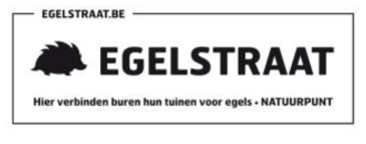
\includegraphics[width=0.6\textwidth]{Images/panneau.png}
    \caption{Panneau \enquote{Egelstraat} reçu une fois que les habitants de la rue ont réussi à connecter 10 jardins}
\end{figure}

\subsubsection{Initiative gouvernementale contre la fragmentation de l’habitat}

Le Vlaams Actieprogramma Ecologische Ontsnippering (VAPEO) est un programme pluriannuel flamand lancé pour lutter contre la fragmentation écologique des habitats naturels. Cette fragmentation est causée par le fait que le réseau routier est l’un des plus dense d’Europe. De plus, il y a la présence de voies ferrées, de canaux et l’urbanisation est intense. Ce programme vise à reconnecter les zones de vie des animaux sauvages via des passages sécurisés (écoducs, écotunnels, bermbruggen/ponts verts, etc.), afin de réduire les mortalités routières (environ 5 millions d’animaux tués par an) et d’améliorer l’accès à la nourriture, aux abris et à la reproduction.

Approuvé en septembre 2020 pour la partie infrastructures routières, le programme couvre initialement la période 2019-2024, mais il est continu, flexible et actualisé en permanence et se poursuit activement au-delà : un suivi est planifié pour 2025-2030, avec un soutien scientifique continu de l’INBO (y compris un monitoring en cours jusqu’en 2026, comme sur la N76).

Piloté conjointement par l’Agentschap Wegen en Verkeer (AWV), le Departement Omgeving (DOMG) et l’Agentschap Natuur en Bos (ANB), il s’appuie sur une base de données des points problématiques (ontsnipperingsdatabank), où chaque nœud est scoré selon des critères écologiques et de faisabilité. La priorité est donnée à 15 goulots d’étranglement majeurs, avec une exécution progressive.

Exemples de projets réalisés ou avancés :
\begin{itemize}
    \item Écopont N75 (Dilsen-Stokkem, Limbourg)
    \item Bermbruggen E19/HSL, E34/E313 et écotunnel E19/A1 (Anvers)
    \item Écopont N76 (Hasselt, Limbourg) : suivi en cours jusqu’en 2026 pour évaluer l’efficacité sur les hérissons et autres espèces
\end{itemize}

Ces mesures restaurent la connectivité écologique, diminuent les collisions et les noyades, et renforcent la viabilité des populations animales. Le VAPEO reste un pilier clé de la politique flamande en terme de biodiversité et d’infrastructures durables en 2026.

\subsubsection{Waarnemingen.be VS Observations.be : Pourquoi cette différence ?}

La comparaison entre `Waarnemingen.be` et `Observations.be` montre immédiatement un déséquilibre marqué en faveur de la Flandre. Cette différence ne reflète pas nécessairement une abondance plus élevée du hérisson au nord du pays, mais plutôt une histoire plus ancienne de mobilisation citoyenne, une base d’utilisateurs plus large et un ancrage plus fort de la culture naturaliste participative.

`Waarnemingen.be`, lancé dès 2008 par Natuurpunt, a bénéficié très tôt d’un réseau dense d’observateurs bénévoles. `Observations.be`, développé plus tard dans le contexte wallon, s’est construit sur une dynamique plus récente. À cela s’ajoutent des facteurs démographiques et territoriaux : la Flandre, plus densément peuplée et plus urbanisée, compte mécaniquement davantage de personnes susceptibles de signaler des observations autour de chez elles, alors que certaines zones wallonnes restent moins couvertes par les observateurs.

Il en résulte une différence importante dans le volume d’informations disponibles. Les cartes issues de ces plateformes montrent une couverture flamande beaucoup plus dense, tandis que la Wallonie présente encore des \enquote{zones blanches}, c’est-à-dire des secteurs où l’absence de données traduit souvent un manque d’observation plutôt qu’une absence réelle de l’espèce. Cette distinction est essentielle, car elle rappelle que l’effort d’observation influence fortement la perception de la distribution du hérisson.

\subsection{Wallonie}

Le recensement du hérisson en Wallonie constitue un enjeu central pour la compréhension et la protection de l’espèce. Plusieurs initiatives ont été mises en place pour mieux suivre l’évolution des populations et sensibiliser le public à leur préservation (Natagora, a). Malgré cela, il reste difficile d’obtenir des données fiables et homogènes, en raison du mode de vie de l’animal, des biais liés à l’observation et des limites propres aux dispositifs de suivi.

Pour commencer, le hérisson est un animal très discret et principalement nocturne. Durant la journée, il reste caché dans des tas de feuilles, des broussailles ou dans les haies, ce qui rend son observation directe relativement rare (Natagora, b). Son repérage dépend donc souvent du hasard. Il est ainsi probable que certains individus ne soient jamais observés ni répertoriés. Par conséquent, la population réelle est souvent sous-estimée.

Ensuite, le recensement repose en grande partie sur la participation citoyenne, ce qui présente certaines limites. Des plateformes d’observation permettent aux citoyens d’encoder leurs observations en indiquant la date, l’heure, le lieu, l’espèce observée, le nombre d’individus et éventuellement une photographie (Natagora, a). Toutefois, les données collectées dépendent fortement du nombre de participants, de leur motivation et de leur répartition géographique. Certaines régions peuvent donc être davantage documentées que d’autres. En Wallonie, une grande partie des observations de hérissons provient par exemple du Hainaut. Cela ne signifie pas nécessairement que les hérissons y sont plus nombreux, mais plutôt que les observateurs y sont plus actifs.

Une autre limite du recensement est liée au fait que les hérissons ne sont pas tous observés dans les mêmes conditions. Les centres de revalidation tels que les CREAVES\footnote{Centre de Revalidation des Espèces Animales Vivant naturellement à l'État Sauvage}  recueillent les hérissons blessés ou affaiblis afin de les soigner avant de les remettre en liberté. Les observations provenant de ces structures concernent donc uniquement des individus en difficulté. Afin de mieux suivre certains individus après leur remise en liberté, des études ont été mises en place en collaboration avec ces centres. Dans certains cas, les hérissons relâchés sont marqués avec une gaine jaune placée sur leurs piquants afin de pouvoir les identifier s’ils sont observés à nouveau. Les citoyens peuvent alors signaler ces individus via les plateformes d’observation, ce qui permet d’obtenir des informations sur leur survie et leurs déplacements après les soins (Ligue Royale Belge pour la Protection des Oiseaux, 2021). Cependant, cette méthode reste limitée car peu d’individus sont marqués et ils ne sont pas toujours revus.

Les données provenant des centres de revalidation montrent également une augmentation importante du nombre de hérissons recueillis. En 2024, plus de 5000 hérissons ont été amenés dans des centres de revalidation alors qu’en 2023 ils n’étaient qu’environ 1500 (Biodiversité Wallonie, 2024). Cette différence importante peut indiquer une augmentation des dangers auxquels l’espèce est confrontée, mais elle ne permet pas de connaître directement la taille totale de la population sauvage.

Enfin, l’analyse des données se complique également en raison de la diversité et de la fragmentation des habitats en Wallonie. Le hérisson peut vivre dans différents milieux tels que les jardins, les zones agricoles ou les parcs. Sa présence dépend de plusieurs facteurs comme la disponibilité de nourriture, la présence de refuges, l’utilisation de pesticides ou encore la présence d’obstacles dans le paysage (Biodiversité Wallonie). Certains équipements domestiques peuvent également représenter un danger, comme les robots tondeuses utilisés la nuit, qui peuvent gravement blesser les hérissons (Service public de Wallonie, 2023). Ces facteurs varient fortement d’un endroit à l’autre, ce qui rend l’interprétation des observations difficile à l’échelle régionale.

Ainsi, les initiatives existantes pour suivre le hérisson en Wallonie — observations citoyennes, données des centres de revalidation et programmes de suivi — restent essentielles pour mieux comprendre la situation de l’espèce et orienter les actions de protection (Natagora, a). Toutefois, le recensement demeure complexe car les données disponibles sont souvent fragmentaires et dépendantes de nombreux biais d’observation, ce qui rend difficile une estimation précise de la taille et de l’évolution des populations.

\subsection{France et Luxembourg}

En France comme au Luxembourg, la collecte de données sur le hérisson repose largement sur la participation citoyenne, mais aussi sur l’implication de structures scientifiques et d’acteurs publics. Les observations sont généralement transmises via des plateformes de recensement, comme iNaturalist. Ce type de science participative est particulièrement utile, car il permet de recueillir un grand nombre d’informations sur une vaste échelle géographique, à condition qu’un travail de validation accompagne ensuite leur exploitation.

En France, ce système est renforcé par des programmes structurés comme Vigie-Nature, coordonné par le Muséum national d'Histoire naturelle. Ces programmes impliquent à la fois des citoyens, des associations naturalistes et des chercheurs, avec des protocoles standardisés pour garantir la qualité des données. Les centres de soins pour la faune sauvage jouent aussi un rôle important, car ils enregistrent des informations précises sur les hérissons recueillis (blessures, causes de mortalité, périodes d’activité), ce qui permet d’avoir une approche complémentaire plus professionnelle.

Au Luxembourg, les mesures mises en place sont particulièrement intéressantes car elles combinent sensibilisation, recherche scientifique et action politique. La campagne \enquote{De Kéisécker}, portée par le Mouvement Écologique, est un exemple de science citoyenne. Elle encourage les habitants à observer et signaler les hérissons, tout en leur fournissant des outils concrets comme des tunnels à empreintes ou des caméras nocturnes. Cette approche permet non seulement de collecter des données, mais aussi de sensibiliser directement la population à la biodiversité locale.

Au niveau institutionnel, le Luxembourg a mis en place une stratégie globale à travers le Plan national pour la protection de la nature (PNPN). Ce plan vise à améliorer l’état de conservation des espèces en agissant directement sur les habitats. Il y a une volonté d’augmenter la disponibilité des habitats favorables en milieu urbain, en développant les espaces verts, en plantant des haies, ou encore en encourageant les jardins plus naturels. L’idée est de recréer des milieux où le hérisson peut se nourrir, se reproduire et se déplacer.

Un point important du PNPN est aussi la réduction des pressions liées aux activités humaines. Cela inclut la diminution de la pollution lumineuse, qui perturbe les espèces nocturnes comme le hérisson, la gestion du bruit, et la limitation de l’usage de pesticides qui réduisent les ressources alimentaires (insectes). Le plan encourage également une gestion différenciée des espaces verts, par exemple en laissant certaines zones non tondues ou en retardant la fauche, afin de créer des refuges pour la faune.

Le Luxembourg cherche à créer des corridors écologiques pour relier les habitats entre eux. Cela est essentiel pour une espèce comme le hérisson, qui se déplace beaucoup mais est fortement impactée par la fragmentation du paysage. Des aménagements comme des passages à faune ou des ouvertures dans les clôtures sont encouragés pour faciliter les déplacements.

En parallèle, le pays s’appuie sur le réseau Natura 2000, qui couvre une part importante du territoire. Même si ce réseau vise surtout des habitats et espèces spécifiques, il contribue indirectement à la protection du hérisson en préservant des milieux naturels de qualité

La recherche scientifique joue aussi un rôle important, notamment avec le Luxembourg Institute of Science and Technology (LIST) et sa division BIODIV. Ces structures utilisent des technologies avancées comme des caméras automatiques, des capteurs ou encore de l’intelligence artificielle pour analyser les données. L’objectif est de combiner les observations citoyennes avec des méthodes scientifiques plus précises, afin d’obtenir une vision globale de l’état des populations.

Enfin, un autre aspect important concerne l’étude des menaces, notamment la mortalité routière. Des relevés sont réalisés pour identifier les zones à risque, et des mesures peuvent ensuite être proposées, comme l’installation de panneaux, la réduction de la vitesse ou la création de passages sécurisés. Ces actions montrent que la conservation du hérisson au Luxembourg ne repose pas seulement sur l’observation, mais aussi sur des interventions sur le terrain.

Globalement, on voit que le Luxembourg adopte une approche assez intégrée : participation citoyenne, cadre politique structuré, recherche scientifique et actions locales. Cette combinaison est intéressante car elle permet d’agir à plusieurs niveaux en même temps, ce qui est essentiel pour une espèce comme le hérisson, fortement impactée par les changements liés à l’urbanisation.

\subsection{Comparaison (vide)}

\subsection{Angleterre}

Au Royaume-Uni, le hérisson occupe une place tout à fait singulière : bien plus qu’un simple animal sauvage, il est devenu une véritable figure emblématique, entre culture populaire et politiques de conservation. Cette popularité ne doit rien au hasard.

Dès le début du XXe siècle, des œuvres comme celles de Beatrix Potter ont largement contribué à façonner l’image du hérisson. Son personnage de The Tale of Mrs. Tiggy-Winkle (1905) présente un hérisson anthropomorphisé, bienveillant et attachant, qui a profondément marqué l’imaginaire collectif britannique (Potter, 1905). Cette représentation culturelle a contribué à faire du hérisson un animal familier et apprécié, transmis de génération en génération (University of Keele, 2018).

Cet attachement s’est confirmé lorsque le hérisson a été désigné \enquote{espèce emblématique du Royaume-Uni} à l’issue d’un vote populaire organisé par BBC Wildlife Magazine où il a obtenu 42 \% des votes(BBC Wildlife Magazine, 2013 ; The Guardian, 2013). Ce choix illustre un lien affectif fort entre les Britanniques et cet animal, d’autant plus présent qu’il fréquente les jardins et les espaces du quotidien.

Dans le domaine de la conservation, cette popularité est pleinement mobilisée. Le hérisson est considéré comme une \enquote{espèce porte-drapeau} (flagship species), capable de sensibiliser le grand public à des enjeux environnementaux plus larges. Comme le souligne la Zoological Society of London, \enquote{connecter les gens à la nature passe souvent par des espèces qu’ils connaissent et apprécient déjà} (ZSL). Le hérisson joue ainsi un rôle clé dans les stratégies de sensibilisation.

Cette dimension affective a des effets concrets : elle favorise la participation aux programmes de science participative, comme les campagnes de recensement ou les initiatives de type \enquote{hedgehog highways}, qui encouragent les citoyens à adapter leurs jardins (PTES). Comme le résument plusieurs programmes britanniques, \enquote{les gens protègent plus volontiers ce qu’ils aiment et reconnaissent}.

Cependant, cette popularité s’accompagne d’un paradoxe : malgré cet engouement, les populations de hérissons ont fortement décliné ces dernières décennies (PTES). Cette situation renforce encore leur statut d’espèce à protéger et agit comme un levier de mobilisation.

Dans ce contexte, l’exemple britannique est particulièrement inspirant pour des projets comme ceux menés en Belgique. Il montre que la réussite d’un recensement ne repose pas uniquement sur des outils scientifiques, mais aussi sur la capacité à créer un lien émotionnel durable avec le public. 

Comme le rappelle Sophie Lund Rasmussen, la conservation du hérisson passe autant par la connaissance scientifique que par l’implication des citoyens et l’amélioration des habitats.

Ainsi, le hérisson devient bien plus qu’un objet d’étude : un véritable vecteur de sensibilisation, dont la popularité peut renforcer l’engagement du public et la participation aux actions de suivi et de protection.

\subsection{Démographie en Belgique}

D’un point de vue démographique, la Wallonie présente une densité de population relativement faible et inégalement répartie. Avec environ 219 habitants par km², elle est moins densément peuplée que les autres régions belges (Statbel, 2023), et sa population se concentre principalement le long d’un axe urbanisé allant de Mons à Liège (Connaître la Wallonie, n.d.). 

Comme le souligne l’Institut wallon de l’évaluation, de la prospective et de la statistique, cette distribution territoriale crée des contrastes importants dans la couverture des données, notamment dans les projets de science participative.

À cela s’ajoute la diversité de la topographie wallonne. Le nord et le centre sont dominés par des paysages agricoles ouverts, tandis que le sud, notamment l’Ardenne, est caractérisé par un relief plus marqué et de vastes zones forestières. Ces dernières occupent une part importante du territoire régional, ce qui influence à la fois l’accessibilité et les conditions d’observation (Service public de Wallonie, n.d.). Or, ces caractéristiques jouent un rôle clé dans le recensement des hérissons.

En effet, ces deux facteurs : densité humaine et topographie, créent un biais important dans la collecte des données. Dans les zones urbaines et périurbaines, les observations sont plus nombreuses, car les volontaires y sont plus présents et les terrains plus accessibles. À l’inverse, dans des régions comme l’Ardenne ou certaines parties de la Lorraine, les données sont plus rares. Cela ne signifie pas nécessairement que l’espèce y est absente, mais plutôt qu’elle est moins observée.

Ce phénomène est bien documenté dans la littérature scientifique. Comme le montrent Dickinson et al. (2010), les données issues de la science participative reflètent autant l’effort d’observation que la réalité écologique. Autrement dit, une zone peu documentée est souvent une zone moins fréquentée par les observateurs, et non une zone pauvre en biodiversité.

Dans ce contexte, les projets portés par Natagora doivent tenir compte de ces biais pour affiner leurs analyses. L’identification de \enquote{zones blanches}, c’est-à-dire de secteurs peu documentés, devient un enjeu stratégique : elle permet de mieux cibler les efforts de recrutement de volontaires et d’améliorer la couverture territoriale du recensement.

Ainsi, en Wallonie, la combinaison d’une faible densité de population, d’une répartition territoriale inégale et d’une topographie contrastée influence fortement la collecte de données sur les hérissons. Ces éléments rappellent que le recensement ne dépend pas uniquement de la présence de l’espèce, mais aussi de notre capacité à l’observer.

\section{Élaboration et utilité d’un prototype}

\subsection{Public cible}

Le projet s’adresse à un public large. Il vise en premier lieu les habitants de Belgique, et plus particulièrement ceux qui disposent d’un jardin ou vivent à proximité d’espaces verts, là où la présence du hérisson est la plus probable.

Une attention particulière a été portée à l’accessibilité du site internet pour les jeunes publics. Le design a été pensé de manière simple, visuelle et intuitive, intégrant des illustrations attractives et des éléments graphiques ludiques. Ces choix permettent de capter l’attention des enfants et des adolescents, tout en facilitant la compréhension des informations. Le quiz proposé sur le site constitue également un outil pédagogique central, permettant d’apprendre à reconnaître les hérissons, à adopter les bonnes pratiques dans les jardins et à mieux comprendre les enjeux liés à leur protection. Ainsi, le projet s’inscrit aussi dans une démarche de sensibilisation et d’éducation à l’environnement.

Par ailleurs, le projet cible également un public plus averti, comprenant les amateurs de nature, les naturalistes, ainsi que les citoyens souhaitant s’impliquer activement dans la collecte de données. Le module de recensement, accessible via le site internet, s’adresse principalement à ces utilisateurs. Il requiert en effet de fournir des informations précises telles que la localisation de l’observation, la date, le type d’observation (directe, individu mort), ainsi qu’une photographie. Ce système permet de garantir une certaine qualité des données collectées, tout en restant accessible à toute personne motivée, même sans formation scientifique approfondie.

Afin d’accroître la visibilité du projet, une stratégie de communication ciblée a également été mise en place. Des flyers ont notamment été distribués au sein de plusieurs associations et structures en lien avec la nature, l’environnement ou la sensibilisation citoyenne. Cette démarche a permis de toucher un public déjà sensible aux enjeux de biodiversité et potentiellement prêt à s’impliquer activement dans le recensement des hérissons.

Enfin, le projet peut également intéresser des acteurs institutionnels et associatifs, tels que des organisations de conservation (par exemple Natagora), des communes ou des initiatives citoyennes locales. Les données collectées via la plateforme ont vocation à être valorisées à plus grande échelle, notamment à travers leur intégration potentielle dans des bases de données existantes ou leur utilisation dans des projets de conservation.

En somme, le projet adopte une approche inclusive combinant sensibilisation, éducation et participation citoyenne.

\subsection{Objectifs du prototype (vide)}

\subsection{Analyse des lacunes des dispositifs existants}

\subsubsection{État des données existantes en Wallonie}

Afin de répondre à la problématique du projet, nous avons d’abord dressé un état des lieux des données disponibles sur le hérisson en Belgique, en particulier en Wallonie. Pour cela, nous avons consulté les principales bases de données d'observations naturalistes accessibles au public, notamment iNaturalist, Observations.be et les plateformes affiliées au réseau GBIF (Global Biodiversity Information Facility).

Ces comparaisons ont permis de mettre en évidence un déséquilibre géographique important : les données relatives aux hérisson d’Europe sont bien plus denses en Flandre qu'en Wallonie. Ce constat confirme les observations rapportées dans la littérature, où une étude spécifique sur la mortalité routière en Flandre a documenté un déclin d'environ 50 \% des individus observés morts sur les routes entre 2010 et 2018. À l'échelle nationale belge, les tendances restent mal quantifiées, l'UICN estimant un déclin de 16 à 33 \% sur 10 ans pour les populations d'Europe occidentale (IUCN, 2024). Dans tous les cas, les effectifs wallons restent largement méconnus faute de données suffisantes.

Plusieurs facteurs permettant d’expliquer ce déficit wallon ont été identifiés :
\begin{itemize}
    \item Il y a une plus petite densité de population humaine dans les zones rurales et forestières de Wallonie. Ce qui réduit logiquement le nombre d'observateurs potentiels.
    \item En Wallonie il y a une sensibilisation moins développée à la science participative.
    \item Il y a l'absence d'une plateforme dédiée, simple et accessible, permettant aux citoyens de signaler facilement leurs observations de manière standardisée et géoréférencée.
\end{itemize}

\subsubsection{Limites des outils existants}

En analysant les plateformes déjà en place, nous avons identifié plusieurs freins à leur appropriation par le grand public. Ces limites sont apparues à la fois dans la littérature et lors de nos propres essais d’utilisation sur le terrain.

Une interface pensée pour les spécialistes, mais peu intuitive pour le grand public. Lorsque nous avons tenté d'importer nos propres observations sur `Observations.be`, nous avons été confrontés à une difficulté récurrente : la plateforme recense un très grand nombre d’espèces, sans mise en avant particulière des enjeux de conservation. Cette richesse est utile pour les naturalistes formés, mais elle peut constituer un obstacle majeur pour un citoyen qui souhaite simplement signaler un hérisson observé dans son jardin. L’utilisateur se retrouve alors face à une masse d’informations et de catégories qui compliquent l’encodage au lieu de le faciliter.

Ce problème est amplifié par le système de classification utilisé. Pour consulter les observations déjà enregistrées, la plateforme demande à l'utilisateur de choisir parmi des groupes taxonomiques tels que les \enquote{Orthoptères}, \enquote{Hyménoptères} ou \enquote{Diptères}. Pour une personne non familière avec la nomenclature scientifique ; c'est-à-dire la grande majorité de la population ; cette terminologie est une barrière et crée de la friction à l’utilisation de ces outils. Il est très difficile, sans être formé, de savoir à quel groupe appartient telle ou telle espèce. Nous avons donc observé que la plateforme est conçue pour un public déjà initié : les naturalistes amateurs avancés ou les professionnels, mais pas pour Monsieur ou Madame tout le monde.

Une faible mise en visibilité des priorités de conservation. Sur les plateformes généralistes, des espèces très menacées apparaissent sur le même plan que des espèces communes, sans hiérarchisation claire des enjeux. Pour le hérisson, récemment reclassé comme espèce quasi menacée à l’échelle européenne, cette absence de mise en contexte dilue le message de sensibilisation. Or, si l’utilisateur ne comprend pas immédiatement pourquoi son observation est utile, il est moins susceptible de participer de façon répétée.

Notre réponse à ces constats a été de concevoir une plateforme dédiée, visuelle et accessible, centrée uniquement sur le hérisson. En se concentrant sur une seule espèce, l’outil gagne en clarté, réduit l’ambiguïté et facilite l’engagement des utilisateurs. L’interface a donc été pensée pour être intuitive, avec une sélection visuelle de l’état de l’animal, un positionnement sur carte interactive plutôt qu’une saisie manuelle des coordonnées, et des catégories d’environnement facilement compréhensibles.

\subsection{Conception du dispositif : le site web les6pics.be}

Sur la base de ces constats, nous avons conçu et développé un site web dédié, accessible à l'adresse \enquote{les6pics.be}. Il a été pensé comme un dispositif ciblant spécifiquement la Wallonie. Chaque choix de conception répond à un problème identifié lors de la phase d'analyse.

\subsubsection{Principes de conception}

Trois principes ont guidé l’ensemble du développement. Le premier, la simplicité d’utilisation : le site doit pouvoir être utilisé sur le terrain, depuis un smartphone, sans connaissance préalable en naturalisme. Le second, la qualité scientifique minimale garantie : le formulaire guide l’utilisateur afin de collecter les informations indispensables à l’exploitation des données. Et enfin, l'attractivité et la fidélisation : des éléments de gamification sont intégrés pour encourager la participation régulière.

\subsubsection{Le module de recensement}

Le c\oe ur du dispositif est le formulaire de recensement, accessible via la rubrique \enquote{Recensement} du site. Il a été conçu pour être rapide, intuitif et utilisable aussi bien sur mobile que sur ordinateur. Cela est une réponse directe aux barrières d'usage des plateformes existantes.

Le formulaire collecte les informations suivantes :
\begin{itemize}
    \item Localisation géoréférencée : l'utilisateur place un marqueur sur une carte interactive (OpenStreetMap), qui renseigne automatiquement les coordonnées GPS et l'adresse approximative. Ce système évite toute saisie manuelle fastidieuse et garantit la précision spatiale des données.
    \item Date de l'observation, pour permettre des analyses temporelles.
    \item État de l'animal, via une sélection visuelle par icônes (vivant, mort sur route, mort hors route, blessé, malade) : ce champ est essentiel pour distinguer les individus actifs des victimes de mortalité routière, l'une des principales causes de déclin documentées.
    \item Type d'environnement (route, zone urbaine, jardin, forêt, parc, haie, champ…), permettant de croiser les observations avec les données d'usage des sols.
    \item Photo optionnelle, pour permettre une validation ultérieure de l'observation.
    \item Notes libres, pour tout élément contextuel supplémentaire.
\end{itemize}

Ce protocole structuré garantit un niveau minimal de standardisation des données, condition nécessaire à leur intégration potentielle dans des bases de données scientifiques existantes.

\subsubsection{La cartographie interactive}

Le site comporte une page \enquote{Cartographie} permettant à tout visiteur de visualiser l’ensemble des observations enregistrées sur une carte de Belgique. Des filtres permettent d’afficher uniquement les données wallonnes ou flamandes, ou encore de ne consulter que ses propres signalements. Une légende distingue également les observations selon leur statut (vivant, mort sur route, mort hors route).

Ce retour visuel immédiat remplit une double fonction. D’une part, il valorise la contribution des utilisateurs en leur montrant l’impact collectif des signalements. D’autre part, il constitue une première interface d’exploration des données pour les chercheurs, associations ou gestionnaires intéressés par la répartition spatiale des observations.

\subsubsection{Gamification et engagement des utilisateurs}

Lors de nos différentes réunions, un constat s’est imposé à nous : la participation citoyenne ne va pas de soi. Dans tout projet de science participative, la difficulté n’est pas seulement de susciter une première contribution, mais de maintenir l’engagement dans la durée. Nous avons donc cherché à comprendre quels mécanismes pouvaient encourager des utilisateurs à revenir régulièrement sur la plateforme.

Pour répondre à cette question, nous nous sommes tournés vers des exemples issus du jeu vidéo et des applications ludiques géolocalisées. Des dispositifs comme \enquote{Pokémon Go} ou le géocaching montrent qu’une activité fondée sur l’exploration d’un territoire peut mobiliser durablement un très grand nombre de personnes. Sans reproduire ces modèles à l’identique, ils montrent qu’une application peut devenir attractive lorsqu’elle combine repères visuels, objectifs clairs et gratification régulière.
\begin{itemize}
    \item des récompenses immédiates et addictives (dopamine via chaque capture) ;
    \item des objectifs concrets servant d’excuse sociale pour sortir ;
    \item une socialisation à faible pression (rencontres fortuites sans obligation d’interagir).
\end{itemize}

La question est alors devenue la suivante : ces principes peuvent-ils être mobilisés dans un cadre non ludique, comme le recensement d’une espèce sauvage ? La littérature sur la gamification apporte des éléments de réponse positifs, en montrant que certains mécanismes issus du jeu peuvent renforcer la motivation, la fidélisation et l’investissement des participants.

La gamification consiste à introduire des logiques ludiques dans un contexte qui ne relève pas du jeu, afin de rendre une activité plus engageante, plus motivante et plus régulière.

Cette intuition a été étudiée dans la littérature scientifique. Une étude publiée dans \textit{Biological Conservation} propose par exemple d’utiliser le potentiel motivationnel de la gamification pour engager les citoyens dans la documentation de la biodiversité locale. Les auteurs soutiennent qu’une telle approche peut accélérer la collecte de données utiles à la recherche et soutenir les décisions de conservation (KC \& Sapkota, 2025).

Une étude consacrée à \textit{Biotracker}, une application mobile gamifiée de collecte de données phénologiques, montre également que ce type de mécanisme peut attirer de nouveaux contributeurs, en particulier parmi les jeunes publics. Les participants se déclaraient notamment motivés par l’obtention de badges et par la comparaison avec leurs pairs, ce qui augmentait leur propension à utiliser l’application (Bowser et al., 2013).

Des exemples concrets issus de la conservation de la biodiversité vont dans le même sens. Des plateformes comme `eBird` ou `iNaturalist` montrent qu’un design centré sur l’utilisateur, associé à des mécanismes de progression et de reconnaissance, peut transformer un simple signalement en pratique régulière et valorisée.

Une étude menée sur la plateforme suédoise Artportalen, qui recense des observations naturalistes sans gamification explicite, souligne a contrario que les utilisateurs, bien que motivés par la curiosité scientifique, n'appréciaient pas l'acte de signalement en lui-même. Ce constat négatif renforce l'intérêt d'intégrer des éléments ludiques pour réduire cette friction perçue (Melin et al., 2020).

Notre approche a donc consisté à réduire la friction d’usage tout en renforçant l’intérêt de la participation. Nous avons cherché à rendre chaque interaction rapide, visuelle et gratifiante. Concrètement, les mécanismes intégrés à notre site sont les suivants :
\begin{itemize}
    \item Un système de badges, attribués en fonction du nombre et de la variété des observations soumises. Ce système  valorise les contributions et crée un sentiment de progression.
    \item Un profil utilisateur permettant de suivre son historique de recensements et de visualiser son impact cumulé sur la carte.
    \item Une \enquote{boutique} de personnalisation d'un avatar hérisson, élément ludique dont la fonction est de créer un attachement émotionnel à l'espèce et à la plateforme.
    \item Un quiz interactif sur la biologie et l'écologie du hérisson, permettant d'apprendre tout en jouant.
    \item Des mini-jeux développés sur Scratch pour enrichir encore l'expérience et toucher un public plus jeune.
\end{itemize}

Il convient enfin de noter que la gamification ne remplace pas la rigueur scientifique : elle en est un levier. En rendant le signalement plus accessible et plus agréable, elle favorise l’augmentation du volume de données collectées, condition essentielle à toute analyse robuste de la distribution du hérisson en Wallonie.

\subsection{Intérêt du prototype dans le cadre du cours (vide)}

\subsection{Usage encadré des outils d’intelligence artificielle}

Dans le cadre de ce projet, des outils d’intelligence artificielle générative, notamment ChatGPT, ont été utilisés de manière ponctuelle et encadrée, en complément du travail réalisé par le groupe.

Ces outils ont principalement servi à soutenir certaines étapes de la rédaction, notamment pour la correction orthographique et grammaticale, l’amélioration de la fluidité du texte et la structuration de certaines idées. Ils ont également été mobilisés de manière ponctuelle pour clarifier la formulation de concepts ou reformuler certains passages afin d’en améliorer la lisibilité.

L’utilisation de ces outils est restée limitée et n’a en aucun cas remplacé le travail de réflexion, d’analyse et de recherche effectué par les membres du groupe. L’ensemble du contenu scientifique, des choix méthodologiques et des interprétations présentés dans ce rapport relève du travail personnel des étudiants.

Par ailleurs, une attention particulière a été portée à la vérification des informations et à la qualité des sources utilisées. Les outils d’intelligence artificielle n’ont pas été employés comme source d’information scientifique, mais uniquement comme un outil d’assistance à la rédaction.

Ainsi, leur utilisation s’inscrit dans une démarche responsable et transparente, conformément aux consignes du cours, tout en garantissant l’intégrité académique du travail présenté.

\clearpage
\nocite{*}
\printbibliography[heading=bibintoc,title={Bibliographie}]

% Fin du document
\end{document}
